\chapter{Performance and other Tips}%
\label{cha:performance_tips}

Performance and usability of Cinelerra are directly related to the software and video format being used in conjunction with your computer system hardware -- the number of CPUs and its speed, I/O bus speed, graphics card, and amount of available memory. A basic, less powerful system will be sufficient for users working with audio only or lower resolution video formats.  Higher end computers will be needed when playing and working with higher resolution formats, like 1080p, 1440p and 2160p. Adding effects and several tracks of audio will require more cpu, memory, and various other resources to read, decode and play video. 

Perhaps the easiest method for determining if your performance could be improved is to look at the numerical value displayed as \textit{Framerate achieved}.  Good performance means that when \texttt{Play every frame} is set in:

\texttt{Settings $\rightarrow$ Preferences, Playback A tab}, the frames/second (frames per second or fps) in playback might be almost always at the maximum rate of your project setting and/or video frame rate. You can check this in \texttt{Settings $\rightarrow$ Preferences, Playback A}, by watching \textit{Framerate achieved} while playing forward.  A higher number is better, up to the format frame rate of the video.

Some hardware considerations are listed here:
\begin{itemize}
	\item Multi-core and more SMP processors greatly improve Cinelerra speed by making use of threads.
	\item A large amount of free memory available can help speed up operations by avoiding unnecessary disk
	swaps and keeping material easily accessible.
	\item Video editing can be quite I/O intensive. If you are going to produce long pieces in uncompressed or
	larger resolution formats, you should have plenty of fast access disk space.
	\item Cinelerra benefits from OpenGL hardware acceleration. A good graphics card is worthwhile to have.
	\item Multiple monitors really come in handy to increase productivity as you can see more information and
	in bigger windows so you do not have to keep moving windows around.
\end{itemize}
Besides the above hardware recommendations, this section covers tips for performance improvements and tips on how to perform some specific tasks, often for older media.

\section{Hardware video acceleration}%
\label{sec:hardware_video_acceleration}

With certain newer, more powerful graphics boards and newer device drivers, there is the potential for enhanced \textit{decode} and \textit{encode} performance.   Decode refers to loading and playing video in Cinelerra. The GPU, Graphics Processing Unit, on the graphics board is accessed via one of the following libraries: vdpau or vaapi. The hardware acceleration done by the graphics card increases performance by activating certain functions in connection with a few of the FFmpeg decoders. This use makes it possible for the graphics card to decode video, thus offloading the CPU.  Decode operations are described here next.  Encode refers to rendering video and is described at the end of this section under \textit{GPU hardware encoding} \ref{sub:gpu_hardware_encoding}

VDPAU, Video Decode and Presentation API for Unix, is an open source library to offload portions of the video decoding process and video post-processing to the GPU of graphics boards, such as Nvidia.  It may also apply to Nouveau and Amdgpu boards (by wrapper), but that has not been verified.

VA-API, Video Acceleration API, is an open source library which provides both hardware accelerated video encoding and decoding for use mostly with Intel (and AMD) graphics boards. 

Currently only the most common codecs, such as MPEG-1, MPEG-2, MPEG-4, and H.264/MPEG-4, are accelerated/optimized by the graphics card to play these particular video formats efficiently. The other formats are not optimized so you will see no performance improvement since the CPU will handle them as before, just as if no hardware acceleration was activated. There are many different graphics cards and computer systems setup, so you will have to test which specific settings work best for you.  So far this has been tested at least with Nvidia, Radeon, and Broadwell graphics boards on some AMD and Intel computers; depending on the graphics card, two to ten times higher processing speeds can be achieved.  However, most graphic operations are single-threaded and may be slower as opposed to multiple CPUs, which frequently multi-thread many operations simultaneously.

\subsection{GPU hardware decoding}%
\label{sub:gpu_hardware_decoding}

\begin{enumerate}
	\item Verify that you have installed \texttt{libva-dev} or \texttt{libva} on your operating system.
	\item Verify that you also have \texttt{libvdpau-dev} or \texttt{libvdpau} installed.
	\item Verify \texttt{Settings $\rightarrow$ Preferences, Playback tab, Video Driver} is set to\texttt{ X11} -- or \texttt{X11-OpenGL} if that	produces better results for your configuration.
	\item Before starting CinelerraGG, you can set an environment variable that can be easily reversed and
	then, to run from the Cinelerra installed directory, key in:
\end{enumerate}

\begin{lstlisting}[language=bash,numbers=none]
CIN_HW_DEV=vdpau ./cin	# for computers with Nvidia and some other graphics cards
CIN_HW_DEV=vaapi ./cin	# mostly for computers with Intel or AMD specific graphics hardware
\end{lstlisting}

If you find that the environment variable setting is advantageous for your CinGG usage and you want to always use it, you can add it to your \texttt{\$HOME} directory \texttt{.profile} file which takes effect every time you log in.  The line you would add would look something like this:

\begin{lstlisting}[language=bash,numbers=none]
export CIN_HW_DEV=vdpau
or
export CIN_HW_DEV=vaapi
\end{lstlisting}

It might be more difficult to analyze problems as a result of using the GPU because of the wide variation in hardware.  When you do not set the \texttt{CIN\_HW\_DEV} environment variable, the code will work exactly as before since this feature is self-contained.

In addition to the environment variable,  there is a \texttt{Settings $\rightarrow$ Preferences, Performance tab, Use HW device} flag with a pulldown to set up \textit{none, vdpau, vaapi,} or \textit{cuda}.  To ensure it takes effect, it is best to set it the way you want, quit out of Cinelerra and then restart.  Its current purpose is for flexibility, but there is a possibility that it might eventually take the place of \texttt{CIN\_HW\_DEV} -- both are not needed.

-- Precedence of the decode hardware acceleration settings are:

-- \texttt{yourfile.opts} is checked first so is of the highest priority; special .opts usage is described below

-- environment variable \texttt{CIN\_HW\_DEV} is checked next

-- preferences \texttt{Use HW device} settings is of the lowest priority

\subsubsection*{Hardware decoding in Cinelerra GG}%
\label{ssub:hardware_decoding_cinelerra}

There are 4 phases during Cinelerra’s handling of hardware acceleration. These first 2 steps occur just \textit{before} the first read.

\begin{enumerate}
	\item Check to see if Hardware Acceleration is enabled, usually indicated by \texttt{CIN\_HW\_DEV} being set to
	vaapi or vdpau.  If enabled, try to activate the decode device, and if that fails revert to software.
	\item The next step is to send some data to decode to see if that works. If this does not work, you will see
	an error message of \textit{HW device init failed, using SW decode}.
\end{enumerate}

\noindent These next 2 steps occur \textit{during} any read.  Now there is no turning back to software so if the hardware gets an error, that video will not be handled correctly.

\begin{enumerate} [resume]
	\item Read the media and send the raw stream data to the device for processing.
	\item Read the device to receive the decoded data, and convert it to the session color model.  If the GPU
	can not convert the data, you will see the error message of \textit{Error retrieving data from GPU to CPU}.
\end{enumerate}

Due to variations in user’s computer hardware configuration, it is often suggested that you refer to your startup window to check for error messages.   Since your situation is unique, the error may not have been seen by anyone else and is probably unknown/undocumented.

\subsubsection*{Possible improvements or differences}%
\label{ssub:possible_improvements_differences}

\begin{enumerate}
	\item The Frames Per Second (FPS) in playback might be mostly at the maximum rate.  You can check
	this in \texttt{Settings $\rightarrow$ Preferences, Playback A}, looking at \texttt{Framerate achieved}; the higher, the better.
	\item Percent of the CPU used should be less, thus saving more CPU for other operations.
	\item Some users get the the impression that playing seems smoother.
	\item The CPU fan noise may go down as the CPU is used less.
	\item The GPU graphics fan noise may go up as the GPU is used more.
\end{enumerate}

Using the GPU is going to react differently depending on your hardware, software, and the number of files loaded. A good way to determine how well it is performing, is to watch the CPU load from another window running the command line routine \texttt{top}. Consider the following possibilities:

\begin{itemize}
	\item If you only use smaller videos occasionally and then use other codecs than the ones mentioned
	previously as being the optimized set, it is usually a better idea to stay with the default settings
	without all the hardware tests.
	\item If you have 4 cores or less, but a really good \textit{gaming card}, using vaapi/vdpau could be a big help.
	\item If you load only a couple of files, the GPU vaapi/vdpau should be faster depending on your graphics
	board and how capable it is.
	\item If you load 10 camera Mixers of H.264 format, it always seems to work a lot better playing them.
	\item If you have an epyc AMD chip with 128 CPUs and load 50 files, without vaapi/vdpau may be better.
\end{itemize}

\subsubsection*{Special .opts file}%
\label{ssub:special_opts_file}

The situation may arise where you have enabled hardware acceleration and after loading several files for a project, you find that a file had some kind of error resulting in a black video instead of an image or you see an error message pop up which states something like \textit{Error retrieving data from GPU to CPU} or \textit{err: Unknown error occurred}. Because the \texttt{CIN\_HW\_DEV} environment variable is either all or none, ordinarily in order to correct the non-working video you would have to turn off hardware acceleration for the entire project/session.  However, there is a way to continue working on your project without having to reload all of your files. You still use the environment variable and it will be effective for all of the formats it is able to handle, but you make an exception for any of the files that erred out. To do this you simply create a file in the same directory with the same name as the erring file with the different extension of .opts. The contents of this .opts file would just be the one line of:

\begin{lstlisting}[language=bash,numbers=none]
cin_hw_dev=none
\end{lstlisting}

Conversely, if you have a bunch of files in your project, like dnxhd format, that are not hardware accelerated, but you have an accompanying large file of type .mp4 for which you would like the hardware acceleration, you can leave the \texttt{CIN\_HW\_DEV} variable unset (that is, do not use it) and just create an .opts file containing the line:

\begin{lstlisting}[language=bash,numbers=none]
cin_hw_dev=vdpau
\end{lstlisting}

For example your file, \texttt{test.mp4}, would have a side-kick called \texttt{test.opts} that will use the GPU for decoding/playing and the other files will just use the software. This is of some advantage because the ones that can not use the GPU if the environment variable is enabled, will not have to even check which saves a minuscule bit of time.

It is important to note that if using the .opts file to override the default \texttt{ffmpeg / decode.opts} file, you will most likely see more warnings (not really errors) in the Cinelerra startup window because the standard \texttt{decode.opts} file has \textit{loglevel = fatal} whereas the default is \textit{loglevel = error}.  To avoid seeing all of the extra warnings, you can simply add the line   \texttt{loglevel=fatal}   to your .opts file.

\subsubsection*{To verify hardware acceleration}%
\label{ssub:verify_hardware_acceleration}

Probably the easiest way to tell if hardware acceleration is working, is just to look at the messages in the window from where you started Cin (not available if start using the application icon).  For example load a png, dnxhd, or some other non-supported format file and you will see messages similar to those below.  The line \textit{HW device init failed, using SW decode} indicates that the vdpau/vaapi HW (hardware) decode is not available so will use SW (software) decode instead.

\begin{lstlisting}[language=bash,numbers=none]
Failed to get HW surface format.
HW device init failed, using SW decode.
file:/tmp/media/aer_zypr.mp4
err: Success

or

Decoder dnxhd does not support device type vdpau.
HW device init failed, using SW decode.
File:/tmp/media/test.gxf
err: Success

or

HEVC with NVIDIA, VDPAU driver is buggy, skipping
\end{lstlisting}

If you would like to see more information on what is occurring, you can modify in the Cinelerra ffmpeg subdirectory, the file:  \texttt{decode.opts}   by temporarily changing the line from \texttt{loglevel =fatal} to \texttt{loglevel =verbose} and restarting Cinelerra.  Then you will see messages in the startup window like:

\begin{lstlisting}[language=bash,numbers=none]
[AVHWDeviceContext @ 0x7fc9540be940] Successfully created a VDPAU device 
(NVIDIA VDPAU Driver Shared Library 390.116 Sun Jan 27 06:28:58 PST 2019) on X11 display :0
[h264 @ 0x7fc950159380] Reinit context to 1920x1088, pix_fmt: vdpau
[h264 @ 0x7fc92c3dd4c0] Reinit context to 1920x1088, pix_fmt: yuv420p
\end{lstlisting}

Again, to measure the performance run \texttt{top} from another window to check the CPU usage which will go lower as more work is offloaded to the GPU graphics card instead (it may go down by 2 to 10 times) or check the \textit{Framerate achieved} while playing.

Some mixed preliminary results that have been reported are provided below.

\subsubsection*{Case 1:}%
\label{ssub:case_1}

\noindent X11 Video Driver set in \texttt{Settings $\rightarrow$ Preferences, Playback A tab}:

\begin{center}
	\begin{tabular}{lcr}
		CIN\_HW\_DEV=off ./cin & &CPU $58\%$ \\
		CIN\_HW\_DEV=vdpau ./cin & &CPU $32\%$ \\
		CIN\_HW\_DEV=vaapi ./cin & &CPU $82\%$ \\
	\end{tabular}
\end{center}

\noindent X11-OpenGL Video Driver set in \texttt{Settings $\rightarrow$ Preferences, Playback A tab}:

\begin{center}
	\begin{tabular}{lcr}
		CIN\_HW\_DEV=off ./cin & &CPU $48\%$ \\
		CIN\_HW\_DEV=vdpau ./cin & &CPU $12\%$ \\
		CIN\_HW\_DEV=vaapi ./cin & &CPU $80\%$ \\
	\end{tabular}
\end{center}

\noindent Best is the least amount of CPU usage. Note that in this case, using X11-OpenGL is better

\subsubsection*{Case 2:}%
\label{ssub:case_2}

\noindent X11 Video Driver set in \texttt{Settings $\rightarrow$ Preferences, Playback A tab}:

\begin{center}
	\begin{tabular}{lcr}
		CIN\_HW\_DEV=off ./cin & &CPU $60\%$ \\
		CIN\_HW\_DEV=vdpau ./cin & &CPU $11\%$ \\
		CIN\_HW\_DEV=vaapi ./cin & &CPU $60\%$ \\
	\end{tabular}
\end{center}

\noindent X11-OpenGL Video Driver set in \texttt{Settings $\rightarrow$ Preferences, Playback A tab}:

\begin{center}
	\begin{tabular}{lcr}
		CIN\_HW\_DEV=off ./cin & &CPU $67\%$ \\
		CIN\_HW\_DEV=vdpau ./cin & &CPU $60\%$ \\
		CIN\_HW\_DEV=vaapi ./cin & &CPU $67\%$ \\
	\end{tabular}
\end{center}

\noindent Best is the least amount of CPU usage. Note that in this case, using X11 is better

Older graphics cards or non-performing graphics cards will probably bring only a small amount of improvement or no speed advantage at all.  You can check to see if vdpau is implemented for your specific Nvidia board at:

\url{https://download.nvidia.com/XFree86/Linux-x86_64/304.137/README/supportedchips.html}

And, you can see what your specific hardware and software might support by running either \texttt{vainfo} or \texttt{vdpauinfo} from the command line.  Partial examples of each are shown below.

\begin{lstlisting}[language=bash,numbers=none]
# vainfo
vainfo: VA-API version: 1.4 (libva 2.4.0)
vainfo: Driver version: Intel i965 driver for Intel(R) Broadwell - 2.4.0.pre1 (2.3.0-11-g881e67a)
vainfo: Supported profile and entrypoints
VAProfileMPEG2Simple            		
...
VAProfileH264Main              
VAProfileH264High  
...
VAProfileH264MultiviewHigh 
VAProfileH264StereoHigh 
...
VAProfileVC1Simple 
...
VAProfileVP8Version0_3 
\end{lstlisting}

\begin{lstlisting}[language=bash,numbers=none]
# vdpauinfo
display: :0   screen: 0
API version: 1
Information string: G3DVL VDPAU Driver Shared Library version 1.0
...
Decoder capabilities:

name                        level macbs width height
----------------------------------------------------
MPEG1                          --- not supported ---                                                                      
MPEG2_SIMPLE           3 65536  4096  4096                                                                       
MPEG2_MAIN               3 65536  4096  4096                                                                       
H264_BASELINE         52 65536  4096  4096                                                                       
H264_MAIN                  52 65536  4096  4096                                                                       
H264_HIGH                  52 65536  4096  4096                                                                       
VC1_SIMPLE                 1 65536  4096  4096                                                                       
VC1_MAIN                     2 65536  4096  4096                                                                       
VC1_ADVANCED         4   65536  4096  4096 
\end{lstlisting}

One last item of note, \textit{nvdec} is also enabled in the ffmpeg build, but at this time it is not known how this decode option on Nvidia graphics boards works or does not work in conjunction with vdpau.

\subsection{GPU hardware encoding}%
\label{sub:gpu_hardware_encoding}

Encoding using hardware acceleration of your graphics board GPU is included in CinelerraGG but it is of limited availability and works only with a specific set of hardware graphics boards, a certain level of graphics driver versions and only with certain ffmpeg formats.  The encoding is done via vaapi (libva installed), which is known to work with Intel HD graphics boards and some others or via nvenc as developed by Nvidia for Nvidia graphics boards.

\subsubsection*{Broadcom, Intel HD, AMD}%
\label{ssub:broadcom_intel_amd}

To use hardware acceleration for rendering (that is, encoding) you do not have to set a preference or an environment variable, as was required for decoding.  To use this feature you use an ffmpeg render options file which specifies a vaapi codec, such as h264\_vaapi.  You must include this line in that options file to trigger the hardware probe: \qquad	\texttt{CIN\_HW\_DEV=vaapi}

There are currently 4 options files available in the Render menu already set up for you that you see when you select the Video wrench and use the down arrow on the first line in the menu.  These are:

\begin{description}
	\item[h264\_vaapi.mp4] known to work on Intel computer with Intel Broadwell graphics driver
	\item[mpeg2\_vaapi.mp4] known to work on Intel computer with Intel Broadwell graphics driver
	\item[mjpeg\_vaapi.mp4] error message of \textit{open failed with mjpeg\_vaapi$\dots$} on above computer
	\item[hevc\_vaapi.mp4] error message of \textit{open failed with hevc\_vaapi$\dots$} on above computer
\end{description}

Other option files can be added as needed for your specific hardware if it is known to work for you, such as VP8 and VP9.  An example of the included Cinelerra’s \texttt{ffmpeg/video/h264\_vaapi.mp4} file (figure~\ref{fig:render-vaapi}):

\begin{lstlisting}[language=bash,numbers=none]
mp4 h264_vaapi
cin_hw_dev=vaapi
profile=high
\end{lstlisting}

\begin{figure}[htpb]
	\centering
	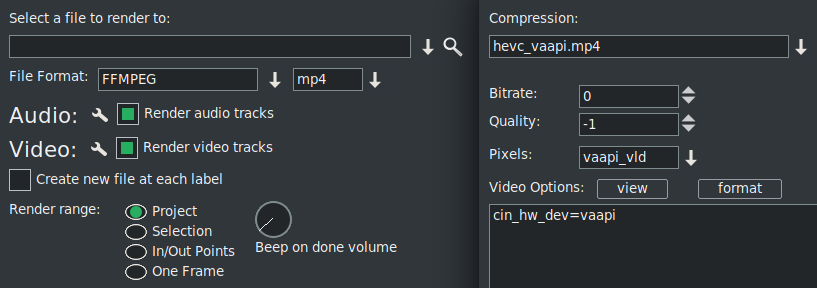
\includegraphics[width=0.8\linewidth]{images/render-vaapi.png}
	\caption{Render menu setup to encode using GPU with vaapi}
	\label{fig:render-vaapi}
\end{figure}

According to an online wiki, hardware encoders usually create output of lower quality than some software encoders like x264, but are much faster and use less CPU. Keep this in mind as you might want to set a higher bitrate to get output of similar visual quality.

Results of a particular test case performed on a Intel, 4-core computer, with Broadwell Graphics using an mp4 input video/audio file with dimensions of

$1440x1080 / 29.97fps$ is shown next (note, filename is \texttt{tutorial.mp4}).  This may very well be a \textit{best case} scenario!  But clearly, at least on this computer with only 4 cores, the hardware acceleration seems to be quite advantageous.  A comparison of the 2 output files using \texttt{ydiff} (as described in Appendix C in the manual) shows no obvious defects.

\begin{center}
	\begin{tabular}{l|cccc}
		&CPU usage & Render Time & File Size & File \\
		\hline
		none & 388\% &100 secs &36,862,542 & h264.mp4 \\
		vaapi & 150\% & 19 secs & 74,522,736 & h264\_vaapi.mp4 \\
	\end{tabular}
\end{center}

\subsubsection*{Nvidia graphics boards}%
\label{ssub:nvidia_graphics_card}

To use hardware acceleration for rendering (that is, encoding) you do not have to set a preference or an environment variable, as was required for decoding.  To use this feature you use an ffmpeg render options file which specifies the nvenc codec, either \texttt{h264\_nvenc.mp4} or \texttt{nvenc.mp4}.  There are several requirements in order for this to work on your computer as listed here:

\begin{enumerate}
	\item Nvidia graphics board at or above a certain hardware level.  For h265, newer boards are required.
	\item Software drivers for your graphics board must be installed on your computer.
	\item The driver must support at least API version 9.0 -- minimum required Nvidia driver for nvenc is
	390.25 or newer.  You will see error messages on the startup window if you are on lower versions.
\end{enumerate}

If you try to render using\texttt{ h264/h265\_nvenc.mp4} formats and do not have an Nvidia graphics card or this feature was not built in, you will see in the window from where you started Cinelerra, the error message: \qquad \textit{Cannot load libcuda.so.1}

A small test using 2 minutes from the 4k version of Big Buck Bunny shows using nvenc can be about 4 times faster.  The test was done on a 4 core Intel laptop with an Nvidia 950M graphics board.

\begin{center}
	\begin{tabular}{l|cccl}
		&CPU usage & Render Time & File Size & File \\
		\hline
		none & 388\% &20 mins 18 secs & 156,517,069 & h264.mp4 \\
		nvenc & 252\% & 5 mins 44 secs & 42,052,920 & h264\_nvenc.mp4 \\
	\end{tabular}
\end{center}

Of note in this test, 388\% CPU usage with only 4 cores shows that there is probably slow down because there is no more CPU power available. Therefore, using the GPU hardware acceleration with nvenc provides a significant speed-up.  Also, note the larger file size without making use of the GPU – this probably indicates that there is a big difference in bitrate or quality parameter settings used in the options file and this should be taken into consideration.

\subsubsection*{Important Tip}%
\label{ssub:important_tip}

There is one last potentially significant graphics speedup when using the X11-OpenGL driver for users with Nvidia graphics boards who are seeing frames/sec achieved lower than what the video format is set to.  You may want to disable \textit{sync to vblank} (an option for OpenGL) in NVIDIA X Server Settings for the proprietary drivers.  This could increase your frames per second on playback.

\subsection{Effects (OpenCL, Cuda)}%
\label{sub:effects_opencl_cuda}

CUDA® is a parallel computing platform / programming model developed by Nvidia that provides big increases in computing performance through use of the GPU. It was first introduced in about 2006 for applications in computationally intense fields such as astronomy, biology, chemistry, and physics.

At the time this was written, the use of Cuda is not going to improve the playing and rendering of video in Cinelerra except in the case where you use a specific Cuda-enabled plugin that is computationally intense -- sadly, most of what Cin does, Cuda will not help.  Cuda is mostly a \textit{block oriented algorithm} which works well for such things as \textit{a flock of birds all flying next to each other}.

The same as for vaapi and vdpau, you can enable Cuda in the\texttt{ Settings $\rightarrow$ Preferences, Performance tab}, \texttt{Use HW Device} but it will not affect anything unless you have Cuda installed on your system and have built Cinelerra yourself with Cuda build enabled.  To install it on your computer, you will need to do the following:

\begin{enumerate}
	\item Make sure you have the Nvidia proprietary library drivers for your graphics board already installed.
	\item Go to the Nvidia Cuda development website and choose one of the available operating system’s
	such as Fedora, OpenSuse, CentOS, Ubuntu, $\dots$ at   \url{https://developer.nvidia.com/}
	\item You will be installing repositories by package -- this will be around 3 GB.
	\item Also, install the Fusion repo, although it is unknown if necessary or not.
\end{enumerate}

There is a very good set of directions on the website to just follow.  Once you have installed the Cuda software on your computer, you must build Cinelerra yourself -- the default build in the configure script for cuda is \textit{auto}.  For Arch, be sure to first key in:     \texttt{setenv CUDA\_PATH=/opt/cuda} 

There are currently 2 available plugins for \textit{show and tell} that take advantage of the hardware acceleration of Cuda -- N\_Body and Mandelbrot as shown next (figure~\ref{fig:cuda-effects}).

\begin{figure}[htpb]
	\centering
	\begin{minipage}[h]{0.99\linewidth}
		\center{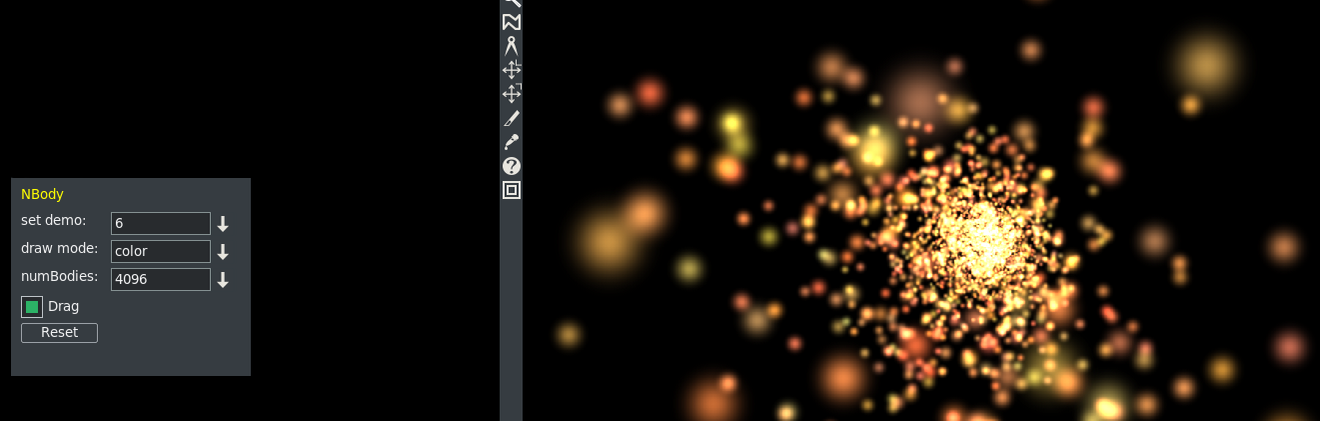
\includegraphics[width=0.99\linewidth]{images/n_body.png}} \\
	\end{minipage}
	\vfill
	\begin{minipage}[h]{0.7\linewidth}
		\center{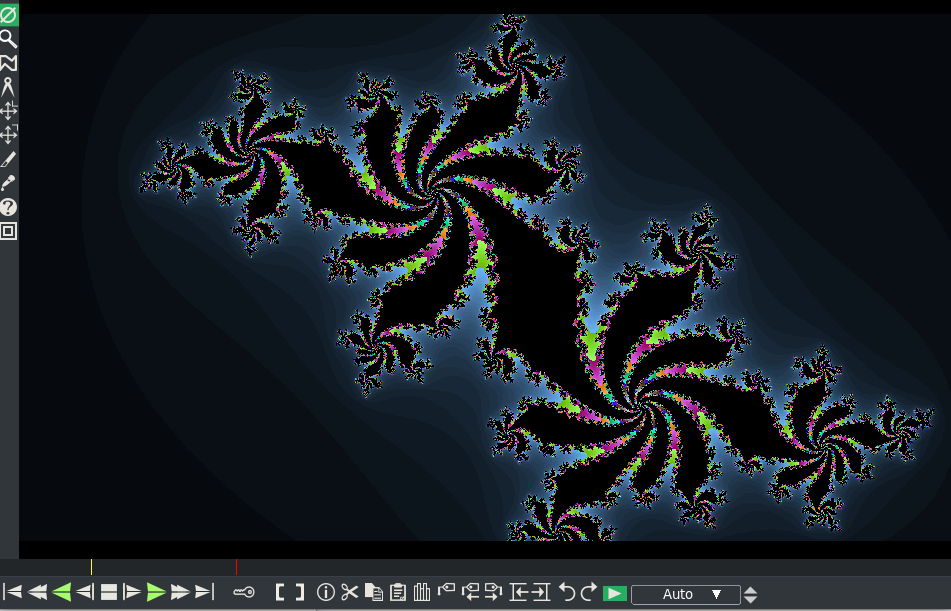
\includegraphics[width=0.99\linewidth]{images/mandelbrot.png}} \\
	\end{minipage}
	\caption{N\_Body and Mandelbrot effects}
	\label{fig:cuda-effects}
\end{figure}

An error you may see on your Cinelerra startup window when you have Cuda installed and try to run one of the 2 plugins is \textit{cudaErrorInsufficientDriver}.  This indicates CUDA 10 (the current version at the time of this writing) is not compatible with the driver version on your computer.  You can either:

\begin{enumerate}
	\item Upgrade the driver if your board supports newer nvidia builds.
	\item downgrade the cuda development package to a version that works for your board.
\end{enumerate}

\subsection{Final Note}%
\label{sub:final_note_on_acceleration}

In wrapping up this Hardware Acceleration section, you may want to refer to the following to determine the current supported formats:

\noindent \url{https://wiki.archlinux.org/index.php/Hardware_video_acceleration}

\section{Optimized Playback -- X11 Direct}%
\label{sec:optimized_playback}

Normally, when Cinelerra reads a video frame, it is copied into a \textit{Vframe}.  This frame may also need other actions performed on it, such as a color model change.  In addition, ffmpeg and libzmpeg \textit{can\_scale\_input}.  So the read can be color transformed and scaled just by asking the library to do that.  This means that if the compositor is in a \textit{good} state with no zoom, the VFrame read can be done in the fastest render color model, and already scaled to the correct size for the compositor.  In reality, this is not what you need for editing, but quite often the \textit{virtualconsole} is not used because the render is media only -- that is \textit{just data}.  If no data transforms are needed and the input scaling can be done, the vrender program detects this, and tells the codec to transmit the data in a compatible way to the compositor canvas. This is the \textit{X11 direct} data path.

With the X11 video driver choice, large format files such as 4K, will playback faster than either X11-XV or X11-OpenGL.  However, you still have the option to turn off the X11 direct data path if you use
\texttt{Settings $\rightarrow$ Preferences, tab Playback A}, set video driver to X11 and uncheck \texttt{use direct X11 render if possible}.


\section{Proxy Settings}%
\label{sec:proxy_settings}

Working with videos that have large image geometry can greatly impede editing.  Instead you can substitute \textit{proxies} which will create smaller video image files from the original file that can then be edited more quickly.   When you are done working on this smaller scale, you will need to bring up the Proxy settings menu again, and change the Scale factor back to the Original size so that all of your edits/work take affect on that original higher quality video on the timeline.  You can not nest clips while in a proxied state; you will get the error \textit{Nesting not allowed when proxy scale $\ne$ 1}.

To use this feature, select \texttt{Settings $\rightarrow$ Proxy settings} and change the Scale factor from Original size to your downsized choice.  You can choose ffmpeg as the File Format and a choice of various codecs associated with that.  A good choice is the default of \texttt{mpeg} which can usually be quite fast.  In addition, to modify values for that codec, click on the wrench icon.  When you have completed your choices, just click \texttt{OK}, and then the video tracks will be rendered. This may take some time, but previous proxy renders will be reused.  The proxy videos will be added to your assets in a separate Proxy folder, and the video track edits will use the proxies.   Proxy downsizing renders all loaded tracks, but only work on the $1^{st}$ video layer of any multi-layer media.  Rendered proxy media is saved in the same directory as the original media.  As usual, you can delete proxy files from the project or disk in the Resources window if you no longer want to retain them.

There are two ways that the proxy files can be used, with or without input scaling. When the proxy is done without rescaling, the Mask, Camera and Projector automations are re-scaled accordingly. In this situation, the entire project will be re-sized so that the session is in the resized geometry.  Not all plugins are useful when the project is rescaled, because the keyframe data must be in the original geometry.  In this case, you can use the rescaler, by enabling \texttt{Use scaler (FFMPEG only)}. This has the added advantage that the project size does not change and the proxy media is down-scaled as usual and up-scaled on read-in, which means the project editing is done in full scale.   Since decoding is done on smaller video, there is a time savings, but all rendering is done full scale.  The main reason for using \textit{scaler} is that it does not change the image coordinate data, so that automation and plugin parameters will be in the original project geometry.   This is not as fast as the first option, but is a performance gain, and may be needed if you are using plugins that need coordinate data such as the Title plugin.  As noted, the scaler only works on ffmpeg video formats.

In the upper right hand corner of the main window, there is a toggle button to easily switch back and forth when you have a proxied file on the timeline.  The icon is to the left of the FF icon.  It will have the letter “P” as the icon for Proxy or if \textit{Using Scaler}, the letter “S”. \quad 
\includegraphics[height=\baselineskip]{images/proxy-01.png} \quad This quick switch is especially useful when editing and you need to see a better image temporarily.

Screencast in figure~\ref{fig:proxy-02} shows the Use scaler checked so you can still use plugins and the original project size is kept.  The Scale factor pull-down gives you available size options.  Note the new media dimensions shown (partially covered).  If the size is an odd number, 1 is added to make the dimensions both even numbers.

In the case of the scaler checkbox, it will retain that setting for ease of use.

\begin{figure}[htpb]
	\centering
	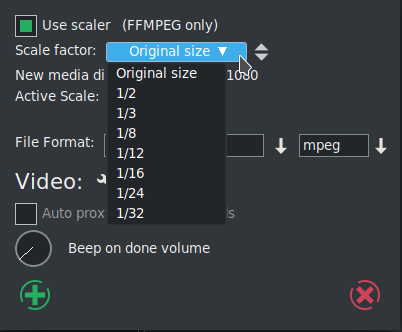
\includegraphics[width=0.8\linewidth]{images/proxy-02.png}
	\caption{Proxy settings dialog}
	\label{fig:proxy-02}
\end{figure}

There is also a convenient \texttt{Beep on done} checkbox included so that you can work on other tasks until there is an audible notify of completion.

A good choice for proxy settings with 1080p source video is:

\begin{lstlisting}[language=bash,numbers=none]
Scale Factor: 	1/4
Use Scaler:	unchecked
File Format:	FFMPEG - mpeg
Video Preset:
Compression:	mpeg.mpeg
Bitrate:	1800000
Quality:	-1
Pixels:		yuv420p
\end{lstlisting}

If you get errors for some videos, such as those with strange variable bit rate or some types of files made on a smartphone, a usually reliable alternative is to change the following parameters:

\begin{lstlisting}[language=bash,numbers=none]
File Format:	FFMPEG - mov
Video Preset:
Compression:	mov.mov
\end{lstlisting}

Or if you want small files with high image quality, a File Format of \texttt{m2ts} is optimal.  For example a 1 GB file can be reduced to 50 MB with scale $\frac{1}{2}$. 

Checking the \texttt{Auto proxy/scale media loads} results in any additional media loads to be automatically proxy scaled.  However, single frame media such as PNG or JPEG \textit{stills}, can not be scaled to \textit{stream} media.  If this type of media exists, you should \texttt{use scaler}.

If you get error messages when creating proxies, check the Video wrench settings.  These usually default to values that are expected to work correctly for the \textit{File Format} and codec you selected but they can be changed and may result in errors.  If you get an error message of \textit{check\_frame\_rate failed} followed by \textit{Error making proxy} in the popup Errors window, do just that and check the Frame rate value by going to the Resources window, Media folder, and use the right mouse button for the Info option for that specific media in question.  You can change the frame rate in this window to a more codec acceptable value.  Different codecs may have different legal values.

More specific information on which plugins need to use scaler is provided here next.  If the keyframe data uses coordinate data that is absolute, then the scaler should be used.  If the data is normalized (like always $0-100\%$) then the proxy can be done without the scaler.  The session geometry format, shown in \texttt{Settings $\rightarrow$ Format} as width x height, is changed if the scaler is not used to cause all of the data to be in the reduced format.  If this affects the plugin operation, then scaler should be used.  Examples of plugins that need the scaler are: Title, AutoScale, Scale, ScaleRatio, and Translate.  Most others are safe to use without scaling.

\section{Some Settings Parameter Values}%
\label{sec:settings_parameter_values}

\texttt{Cache} in \texttt{Settings $\rightarrow$ Preferences, Performance tab} is used to store images on the timeline.  One 1080p frame uses about 10 MB.  The default setting is 256 and this is enough for testing and running.  However, why not use more memory if it is available.   To experiment for testing a good number tuned to the way you use your computer, set the cache to 0, start up Cinelerra, load a typical media file, play it and run \texttt{top} on the command line in another window to see how much memory is being used.  In the \textit{top} display, look at \textit{free} memory.  Whatever your computer is not using, is a good number to use for cache.  If you start other programs, or change the design of the session so that it uses a lot of frame storage, you may need to experiment again later and resize accordingly.

For system \textit{swap}, 1 GB seems to be more than sufficient.  If the amount of memory being used by the program is \textit{close}, then swap might save you but often if swapping becomes necessary, it presents more problems and you end up killing the Cinelerra process anyway.

\section{Tips for Improving Smaller Computers Use}%
\label{sec:tips_improving_smaller_computers}

A list of items to check for smaller computers that will help to use less cpu/memory/resources follows:

\begin{itemize}
	\item For large media files, use proxy to do your main editing.
	\item In \texttt{Settings $\rightarrow$ Preferences, Appearance tab}, uncheck \textit{Use thumbnails in resource window}.
	\item In \texttt{Settings $\rightarrow$ Preferences, Appearance tab}, uncheck \textit{Autocolor assets}.
	\item  Speed-up certain time-consuming FFmpeg plugins through use of a carefully selected \texttt{.opts} file.
	\item For large media files, in \texttt{Settings $\rightarrow$ Preferences, Playback A}, Video Driver set \textit{use direct X11 render if possible}.
	\item For the Video Driver in \texttt{Settings $\rightarrow$ Preferences, Playback A}, if using a good graphics card, choose \textit{X11-OpenGL}.
	\item Set \textit{CIN\_HW\_DEV=vdpau} or \textit{vaapi} to use the graphics GPU for certain ffmpeg media decoding.
	\item If you have multiple cpus or multiple computers, even if slow, take advantage of using \textit{Render Farm}.
	\item When editing, \textit{background rendering} causes temporary output to be rendered constantly while the
	timeline is being modified. The temporary output is displayed during playback whenever possible so 
	it does not have to be recalculated -- very useful for transitions and previewing effects that are slow.
	\item In  \texttt{Settings $\rightarrow$ Preferences, Playback A}, uncheck \textit{Play every frame} which means frames will be skipped as playback of the video falls behind.
	\item Adjust \textit{Cache size} in \texttt{Settings $\rightarrow$ Preferences, Performance tab}, to not exhaust the memory and yet still provide decent playback.
\end{itemize}

\section{General Crash Handling Tips}%
\label{sec:general_crash_tips}

This section is a handy guide for describing various kinds of software computer system failures.  Only some of these various lockups or crashes can be dealt with.  Hopefully, it will help to have some hints to know what kind of failure it is, or to save your work or to avoid future problems.  For most of this, your user name must be root, although you can certainly try to see if it works for you when not root.

\begin{description}
	\item[System lockups:] When the system locks up, it is usually a system problem.  Normally an application program cannot lock up the system.  It is a major goal of system design to prevent an application (app) from failing a system interface.  This does not mean an app can not cause a system lockup, but it is unusual.
	\item[Cinelerra crash:] This is covered in  \ref{cha:Crash Dumps for Analysis} Crash Dumps for Analysis, chapter 18.  Just a reminder that for best results you should be root and by providing a crash dump and as much other information as possible, you will be helping the developer to analyze the problem and fix it so that it can be avoided in the future.
	\item[X Server crash:] Keyboard does not respond, screen is frozen, caps lock may operate LED light.  Sometimes using \texttt{ctrl-alt-F1} $\dots$ \texttt{ctrl-alt-F7} (etc.) will allow you to regain control of a VT console.  You can use this to login and check logs: eg. \textit{/var/log/Xorg.0.log}, \textit{dmesg}, \textit{journalctl} $\dots$ etc.  If you have another computer, make sure a terminal server is configured (for example: rsh, ssh, or telnet), then remote login via this other computer and check the logs.  Most important is to immediately note the current software state, and the very last thing that preceded the crash, i.e. last button click, last keystroke, $\dots$ or whatever.
	\item[Kernel crash:] The machine goes completely dead.  The keyboard caps lock LED will probably be flashing.  Most likely the only way to see anything after the kernel crashes is to use a serial port console log and usually kdb, the kernel debugger, and special cabling.  This requires a lot of setup, and is normally reserved for experts.  Login from another computer will not work.  Pinging the ip address will not respond since the network stack is part of the kernel.  There are some virtual machine setups that will let you debug a \textit{guest} kernel, but this also requires a lot of setup, and affects which kernel is currently under test.  The kdb route is preferable.
	\item[Keyboard grabs, Server grabs, and Deadlocks:] A grab is an X-server state where all events are forced to just one window event stream.  This forces the user to respond to the dialog.  Things seems to be working, but no keypresses do anything useful. The system clock and other programs will still be working.  The network will work for remote logins. Grabs can be canceled if the \texttt{/etc/X11/xorg.conf} X config contains special setup as shown below:
\end{description}

\begin{lstlisting}[language=bash,numbers=none]
Section "ServerFlags"
	Option      "HandleSpecialKeys" "Always"
	Option      "AllowDeactivateGrabs" "True"
	Option      "AllowClosedownGrabs" "True"
EndSection

Section "InputDevice"
	Identifier  "Keyboard"
	Driver      "evdev"
	...
	Option "XkbOptions" "terminate:ctrl_alt_bksp"
	Option "XkbOptions" "grab:break_actions"
EndSection
\end{lstlisting}

or to \texttt{\$HOME/.xinitrc}, add:

\begin{lstlisting}[language=bash,numbers=none]
#  xkb terminate/grab actions disabled in xorg.conf, use:	
setxkbmap -option "grab:break_actions"
setxkbmap -option "terminate:ctrl_alt_bksp"
ctrl-alt-bksp = terminate the X-server, may restart automatically
\end{lstlisting}


Modal forms (always on top, and usually ptr/kbd grab) dialog boxes can lock a system by putting a form over another form holding a grab.  This means the form that needs input may never get any because you can not get to it, and the result is a deadlock.  Usually you will have to restart X (\texttt{ctrl-alt-bksp}).

\begin{description}
	\item[Window Manager issues:] The \textit{desktop} window manager can intercept and modify all kinds of user input.  Mostly, this is a good thing, but can be a nuisance.  If user keypresses can be programmed to trigger actions, then they may be useful to send \texttt{KILL} or \texttt{INTR} to an app that seems to be holding X's attention.  For example:
	\begin{lstlisting}[language=bash,numbers=none]
	killall -INTR cinelerra,
	killall -9 cinelerra,	
	killall X,
	# but you must run as root to be able do this
	\end{lstlisting}
	The \texttt{ALT} and \texttt{META} keys may be intercepted by the window manager, and this can cause unexpected interface operations.
\end{description}

\section{Tips for Specific Operations}%
\label{sec:tips_specific_operations}

\subsection{Generating a 440 Hz tone}%
\label{sub:generating_440_tone}

To create a specific 440 Hz tone, follow these steps.  You can vary the length, use more channels, or change the frequency to a different desired value (figure~\ref{fig:aeval}).

\begin{enumerate}
	\item Make sure there is an armed audio track on the timeline, get into Cut and Paste mode, and highlight
	a selection or define In/Out points where you want to insert the audio tone.
	\item Go to \texttt{Audio $\rightarrow$ Render effect}.  Rendered effect usage is described in Effect Plugins (\ref{sec:rendered_effects}), chapter 10. This brings up a menu where you will select the desired effect which in this case is \textit{F\_aeval}.  Also Select a file to render to, a File Format, and Insertion strategy of Paste at insertion point.
	\item Click on the green \texttt{OK} checkmark which will popup the F\_aeval effect so that you can set the
	parameters.
	\item Highlight the \texttt{exprs} option and key in a specific audio filter expression which for 440 Hz would be:
	$\sin(2\pi t\times440)$.  Then hit the \texttt{Apply} button.
	\item Next when you hit the green \texttt{OK} checkmark on the Cinelerra: Effect Prompt popup, you will have
	your 440 Hz tone on the timeline plus in the select file that you chose to render it to.
	\item To use 2 channels instead of 1, in the F\_aeval menu highlight the \texttt{channel\_layout} option and change
	that to 1C|2C instead of the usual default of 1C.
\end{enumerate}

\begin{figure}[htpb]
	\centering
	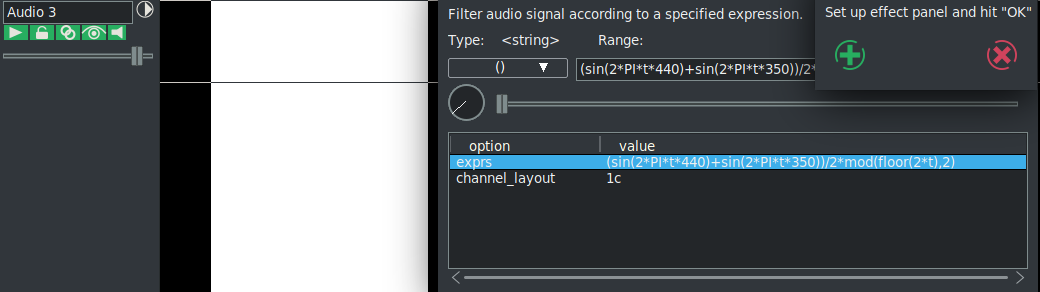
\includegraphics[width=1.0\linewidth]{images/aeval.png}
	\caption{Use Audio$\rightarrow$Render effect to set render parameter values and then that effect can be varied.}
	\label{fig:aeval}
\end{figure}

\subsection{Camera supplied LUTs}%
\label{sub:camera_supplied_luts}

A LUT, acronym for Look-Up Table, is a mathematically precise way of taking specific RGB image values from a source image and modifying them to new RGB values by changing the hue, saturation and brightness values of that source image. In other words, LUTs are used to map one color space to another.  Some high-end cameras supply a \texttt{.cube} file to use as input. There are several different ffmpeg plugins included with CinGG for using Lut's.  These are:

\begin{description}
	\item[F\_lut:] Compute and apply a lookup table to the RGB/YUV input video.
	\item[F\_lut1d:] Adjust colors using a 1D LUT.
	\item[F\_lut3d:] Apply a 3D LUT to an input video.
	\item[F\_lutrgb:] Compute and apply a lookup table to the RGB input video.
	\item[F\_lutyuv:] Compute and apply a lookup table to the YUV input video.
\end{description}

For example, to use a 3dlut simply load your video, drop the F\_lut3d plugin on that track, and bring up the lut3d controls window, highlight the \texttt{file} option, key in your file name (whit path), and hit \texttt{apply} to have the lut take effect.  To easily adjust, move the \texttt{fader} slider in the patchbay for that video track.

\subsection{Encoding into Dolby Pro Logic}%
\label{sub:encoding_dolby_pro_logic}

Dolby pro logic is an easy way to output 6 channel audio from a 2-channel soundcard with degraded but useful results. Rudimentary Dolby pro logic encoding can be achieved with usage of some effects.

\begin{enumerate}
	\item First, create the front left and right channels. Create 2 audio tracks, each carrying either the left or
	right channel. Pan the left channel to the left and the right channel to the right with the pan control.
	\item Now create the rear left and right channels. Create another 2 audio tracks as above -- the left channel
	panned left and the right channel panned right. Then apply invert audio to both new channels and
	the signals will come out of the rear speakers.
	\item Next, create the center channel by creating a single audio track with monaural audio from a
	different source. Center it with the pan control and the signal will come out of the center speaker.
\end{enumerate}

\begin{itemize}
	\item If a copy of the signal in the back speakers is desired in any single front speaker, the signal in the back
	speakers must be delayed by at least $0.05$ seconds and a single new track should be created. Pan the
	new track to orient the signal in the front speakers.
	\item If the same signal is desired in all the speakers except the center speaker, delay the back speakers by
	$0.5$ seconds and delay either the front left or front right by $0.2$ seconds.
	\item If you want to hear something from the subwoofer, create a new track, select a range, drop a
	synthesizer effect, and set the frequency below $60 Hz$. The subwoofer merely plays anything below
	$60Hz$ or so.
\end{itemize}

Other tricks you can perform to separate the speakers are parametric equalization to play only selected ranges of frequencies through different speakers and lowpass filtering to play signals through the subwoofer.

\subsection{Improving Analog TV Quality}%
\label{sub:improving_tv_quality}

The picture quality on analog TV is not always good but you can modify parameters in Cinelerra to make it look more like it did in the studio.

First, when capturing the video, capture it in the highest resolution possible. For Europeans this would be $720\times576$ and for North Americans, $720\times480$. Do not adjust the brightness or contrast in the recording monitor, but you might want to max out the color. Capture the video using MJPEG or uncompressed Component Video if possible; if not possible, then capture it using JPEG preferably or RGB if that is all that will work.  Now on the timeline use Settings $\rightarrow$ Format to set a YUV colorspace, drop a \textit{Downsample} effect on the footage and set it as follows:

\begin{lstlisting}[language=bash,numbers=none]
Horizontal:					2
Horizontal offset: 	0
Vertical:						2
Vertical offset: 		0
	 red
x  green
x  blue
	 alpha
\end{lstlisting}

Use the Camera in the compositor to shift the picture up or down a line to remove the most color interference from the image. If you have vertical blanking information or crawls which constantly change in each frame, block them out by using a Mask. This improves compression ratios.   More invasive quality improvement techniques involve removing the interlace via deinterlacing.

\subsection{Remove Interlacing}%
\label{sub:remove_interlacing}

Interlacing often exists on older video sources, such as camcorders, and was previously used in broadcast television. Playing this video results in jagged images on a computer monitor, but with Cinelerra you can use deinterlacing effects to solve this.  After some experimentation, it has been determined that the FFmpeg \texttt{F\_kerndeint} plugin seems to produce the best results with the least amount of fiddling.  But some of the parameters described next are pertinent to other potential plugin usage.

\begin{description}
	\item[Line Doubling:] done by the \texttt{Deinterlace} effect when set to \textit{Odd} lines or \textit{Even} lines.  When applied to a track it reduces the vertical resolution by $\frac{1}{2}$ and gives you progressive frames with stairstepping. This is only useful when followed by a scale effect which reduces the image to half its size.
	\item[Line averaging:] the \texttt{Deinterlace} effect when set to \textit{Average even} lines or \textit{Average odd} lines does exactly what line doubling does except instead of making straight copies of the lines, it makes averages of the lines. This is actually useful for all scaling.
	\item[Inverse Telecine:] this is the most effective deinterlacing tool when the footage is an NTSC TV broadcast of a film. It is described in Effect Plugins (\ref{sub:inverse_telecine}), chapter 10.
	\item[Time base correction:] the previously discussed three tools either destroy footage irreversibly or do not work at times. Time base correction may be a better tool to use because it leaves the footage intact. It does not reduce resolution, perceptually at least, and does not cause jittery timing.
	\item[Frames to Fields effect:] converts each frame to two frames, so it must be used on a timeline whose project frame rate is twice the footage's frame rate. In the first frame it puts a line-averaged copy of the even lines. In the second frame it puts a line-averaged copy of the odd lines. When played back at full framerate it gives the illusion of progressive video with no loss of detail. This effect can be reversed with the Fields to Frames effect, which combines two frames of footage back into the one original interlaced frame at half the framerate. However, keep in mind that Frames to Fields inputs frames at half the framerate as the project. Effects before Frames to Fields process at the reduced framerate.  The output of Frames to Fields can not be compressed as efficiently as the original because it introduces vertical twitter and a super high framerate. Interlaced $29.97$ fps footage can be made to look like film by applying Frames to Fields and then reducing the project frame rate of the resulting $59.94$ fps footage to $23.97$ fps. This produces no timing jitter and the occasional odd field gives the illusion of more detail than there would be if you just line averaged the original. It is described in Effect Plugins (\ref{sub:frames_to_fields}), chapter 10.
	\item[HDTV exceptions:] $1920\times1080$ HDTV is encoded in a special way. If it is a broadcast of original HDTV film, an inverse telecine works.  But if it is a rebroadcast of a $720\times480$ source, you need to use a time base and line doubling algorithm to deinterlace it.
\end{description}

\subsection{Making video look like film}%
\label{sub:making_video_look_film}

With an older camcorder video which has low quality video, you can improve the results by turning it into progressive 24 fps output as close as possible.  Only do this for low quality video.

\begin{enumerate}
	\item Set project framerate to twice the video framerate.
	\item Apply a \texttt{Sharpen} effect. Set it to sharpness: 25, no interlacing, and horizontal only.
	\item Drop a \texttt{Frame to Fields} effect on the same track. Set Average Empty Rows to on and play through 
	the video a few times to figure out which field is first. If the wrong field is first, the motion is shaky.
	Any editing in the doubled frame rate may now damage the field order. It is not clear which is the
	easiest way to support warnings for field glitches but you should go back to the normal framerate to
	do editing or play test to make sure the fields are right.
	\item Render just the video to the highest quality file possible.
	\item Import the video back to a new track. Set the project framerate to 24. The new track should now
	look more like a file with sharper images than the original footage.
\end{enumerate}

This entire procedure could be implemented in one non-realtime effect, but the problem with that is you will most often want to keep the field based output and the 24 fps output for historical purposes. A non-realtime effect would require all that processing just for the 24 fps copy.

\subsection{Clearing out haze}%
\label{sub:clearing_out_haze}

If you photograph a lot of haze instead of blue sky, these horizon shots will usually need more depth. You can use the \texttt{gradient} effect to improve your video. Drop the gradient effect on hazy tracks and set the following parameters:

\begin{lstlisting}[language=bash,numbers=none]
Angle: 				0
Inner radius: 0
Outer radius: 40
Inner color:  blue 100% alpha 
Outer color:  blue 0% alpha
\end{lstlisting}

It is important to set the $0\%$ alpha color to blue even though it is $0\%$ alpha. The color of the outer alpha is still interpolated with the inner color. This is a generally applicable setting for gradient. Some scenes may work better with orange or brown for an evening feel.

\subsection{Making a ringtone for a cell phone}%
\label{sub:make_ringtone_phone}

\begin{enumerate}
	\item Go to \texttt{File $\rightarrow$ Load files$\dots$} and load a sound file with Insertion strategy: \textit{Replace current project}.
	\item Go to \texttt{Settings $\rightarrow$ Format }change \textit{Channels} to 1 and \textit{Samplerate} to 16000 or 22050.
	\item Highlight a region of the timeline to use for the ringtone. To improve sound quality on the cell
	phone, you need the maximum amplitude in as many parts of the sound as possible.
	\item Right click on track Audio 1 and select \texttt{Attach effect}. Highlight the \textit{Compressor} effect and hit
	\texttt{Attach} in the attachment popup.
	\item Make sure the insertion point or highlighted area is in the region with the Compressor effect.
	\item Right click on track Audio 2 and select \texttt{Attach effect}.
	\item Highlight Audio 1 Compressor and hit \texttt{Attach}.
	\item Click the Audio 1 Compressor's magnifying glass to bring up the compressor GUI.
	\item Set the following parameters:
	\begin{lstlisting}[language=bash,numbers=none]
	Reaction secs: -0.1
	Decay secs: 0.1
	Trigger Type: Total
	Trigger: 0
	Smooth only: No
	\end{lstlisting}
	\item Click Clear to clear the graph. Click anywhere in the grid area and drag a new point to 0 Output
	and -50 Input. The graph should look similar to the figure~\ref{fig:ringtone}.
	\item Go to \texttt{File $\rightarrow$ Render}. Specify the name of an mp3 file to output to. Set the file format to MPEG
	Audio. Click the wrench for Audio and set Layer to III and Kbits per second to 24 or 32. Check
	Render audio tracks and uncheck Render video tracks. Hit OK to render the file.
\end{enumerate}

\begin{figure}[htpb]
	\centering
	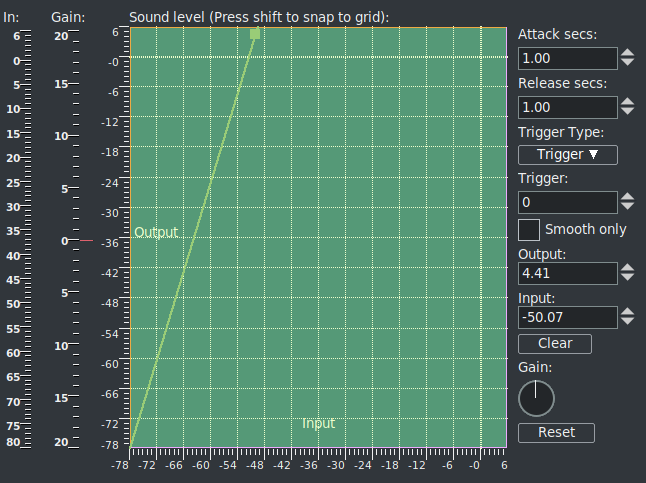
\includegraphics[width=0.8\linewidth]{images/ringtone.png}
	\caption{Using the Compressor plugin graph to create a ringtone}
	\label{fig:ringtone}
\end{figure}

The resulting .mp3 file can be uploaded to a web server and then the phone's web browser can download the .mp3 file directly from the URL. There may be a size limit on the file.

\subsection{Time stretching audio}%
\label{sub:time_stretching_audio}

It may appear that time stretching audio is a matter of selecting a region of the audio tracks, enabling recording for the desired tracks, going to\texttt{ Audio $\rightarrow$ Render Effect}, and applying \textit{TimeStretch}. In actuality there are 3 audio effects for time stretching: Time Stretch, Resample, and Asset info dialog.

\textit{Time Stretch} applies a fast Fourier transform to try to change the duration without changing the pitch, but this introduces windowing artifacts to the audio. It is only useful for large changes in time because obvious changes in duration make windowing artifacts less obtrusive.

For smaller changes in duration, in the range of $5\%$, \textit{Resample} should be used. This changes the pitch of the audio but small enough changes are not noticeable. Resample does not introduce any windowing artifacts, so this is most useful for slight duration changes where the listener is not supposed to know what is going on.

Another way to change duration slightly is to go to the Resources window, highlight the media folder, right click on an audio file, click on \textit{Info}. Adjust the sample rate in the Info dialog to adjust the duration. This method also requires left clicking on the right boundary of the audio tracks and dragging left or right to correspond to the length changes.

\subsection{Pan and zoom: still images}%
\label{sub:pan_zoom_still_image}

Cinelerra's powerful keyframe features allow you to use pan and zoom effects on still pictures.

\begin{enumerate}
	\item Load and create a clip from a still image. Make the clip 10 seconds long.
	\item Activate the automatic generation of keyframes.
	\item Using the transport controls, go to the beginning of the clip.
	\item Using the compositing camera control set the clip's initial position.
	\item Using the transport controls, move forward a couple of seconds on the clip.
	\item Dragging on the compositing camera, move the camera center to a new position further along.
	\item Next go to the beginning of the clip and play it.
\end{enumerate}

You can see that the camera smoothly flows from keyframe point to next keyframe point, as Cinelerra automatically adjusts the camera movement in straight lines from point to point.

